\documentclass[12pt]{report}

\usepackage{geometry}
\usepackage{hyperref}
\usepackage{listings}
\usepackage{amsmath}
\usepackage{graphicx}
\usepackage[english]{babel}

\hyphenation{hard-ware}
\hyphenation{in-for-ma-tion}
\hyphenation{in-ter-pret-ing}
\hyphenation{mul-ti-plica-tive}
\hyphenation{con-trollers}
\hyphenation{seam-less-ly}
\hyphenation{func-tion-al-i-ty}
\hyphenation{tem-per-a-ture}
\hyphenation{be-gin-ning}
\hyphenation{cre-ation}
\hyphenation{func-tion-al-i-ties}
\hyphenation{im-ple-men-ta-tion}
\hyphenation{con-trol}
\hyphenation{ref-er-ence}
\hyphenation{ex-per-i-ment}
\hyphenation{Te-Co-Lab}
\hyphenation{Transfer-Function}

\geometry{a4paper, total={170mm,257mm}, left=20mm, top=20mm}

\title{TeCoLab: Temperature Control Laboratory \\ User Manual}
\date{}

\begin{document}
\maketitle
\tableofcontents

\chapter{Getting Started}\label{chap:getstarted}

\section{What is TeCoLab?}\label{sec:WhatIsTecolab}

TeCoLab, short for Temperature Control Laboratory, is an open-source tool comprising hardware, firmware and software. It is designed for experimenting with control algorithms in the context of temperature control. You can access all the project files on our \href{https://github.com/ytcsc/TeCoLab/tree/main}{GitHub repository}. Before delving into the details, let's embark on a step-by-step tutorial to implement a discrete-time PI (Proportional-Integral) controller with period of 1 second. Our objective is to regulate the temperature of Heater 1 to 15 °C above ambient temperature.

\section{What do I need to run TeCoLab?}

\noindent \textbf{Hardware:}
\begin{itemize}
    \item \textbf{TeCoLab hardware:} You can assemble your own TeCoLab using the files and information available on our GitHub repository;
    \item \textbf{Arduino Nano:} The microcontroller used in this project;
    \item \textbf{USB-B cable:} The standard communication cable for the Arduino;
    \item \textbf{12 V DC power supply:} A 12 V DC power supply with at least 2 A current capacity. Connect the power supply to jack J1 (with positive in the middle) or the bornier terminal J2.
\end{itemize}

\noindent \textbf{Software:}
\begin{itemize}
    \item \textbf{TeCoLab files:} Download from our GitHub repository;
    \item \textbf{Python 3:} Used to execute the TeCoLab program;
    \item \textbf{Python 3 dependencies:} Refer to the list in Chapter~\ref{chap:dependencies};
    \item \textbf{Arduino software:} Required for loading the firmware to your Arduino (you will only need to perform this once);
    \item \textbf{Spreadsheet editor:} A spreadsheet editor, such as LibreOffice Calc, will be useful.
\end{itemize}


\section{Downloading TeCoLab}

To obtain TeCoLab, follow these steps:

\begin{enumerate}
    \item Visit the TeCoLab GitHub repository, click on ``Code" and select ``Download ZIP";
    \item Unzip the downloaded content;
    \item Voilà! TeCoLab is now on your computer.
\end{enumerate}

\section{Programming Your Arduino}

In the folder \texttt{TeCoLab/Firmware} you'll find the firmware project named \emph{Firmware.ino}. Follow these steps to program your Arduino:

\begin{enumerate}
    \item Open the \emph{Firmware.ino} project using the Arduino software;
    \item Load the firmware into your Arduino;
\end{enumerate}

No changes are needed in the firmware. This procedure is a one-time procedure.

\section{Important Files of TeCoLab}

Three files are crucial in TeCoLab:

\begin{itemize}
    \item \textbf{Experiment File:} A \texttt{.csv} file located in \texttt{TeCoLab/Software/Experiments}. In this file, you will define your experiment, including setpoints of temperature, desired disturbances, etc.
    \item \textbf{Control File:} A \texttt{.py} file located in \texttt{TeCoLab/Software/Controllers}. In this file, you will define the control algorithm you want to test during the experiment.
    \item \textbf{Log File:} A \texttt{.csv} file. After defining the experiment and control files, you can execute an experiment. TeCoLab will record the data, such as the temperature evolution, in a log file saved at \texttt{TeCoLab/Software/Logs}.
\end{itemize}

For more information about these files, refer to Chapter~\ref{chap:files}.


\section{Creating Your Experiment}

Let's create our first experiment, aiming to regulate the temperature of Heater 1 to 15 °C above the ambient temperature, as mentioned in Section~\ref{sec:WhatIsTecolab}.

\begin{enumerate}
    \item Navigate to \texttt{TeCoLab/Software/Experiments}.
    \item Copy the file \emph{Template.csv} and rename it to \emph{MyFirstExperiment.csv}.
    \item Open the file. Although the header (first row) contains various fields, we will focus on only two: \texttt{TIME} (first column) and \texttt{SP1\_REL} (fourth column).
    \item Edit your file to resemble the example in Table~\ref{tab:ExpFileExample}. It will end with only three rows (besides the header). Do not fill in any other fields besides those specified in the example.
\end{enumerate}

\begin{table}[!htbp]
    \centering
    \begin{tabular}{|c|c|c|c|c|c|c|}
    \hline
    TIME & SP1\_ABS & SP2\_ABS & SP1\_REL & SP2\_REL & $\ldots$  \\ \hline
    0 & & & 0 & & $\ldots$ \\ \hline
    5000 & & & 15 & & $\ldots$ \\ \hline
    900000 & & & 0 & & $\ldots$ \\ \hline
    \end{tabular}
    \caption{Setting up your experiment file.}\label{tab:ExpFileExample}
\end{table}

In the experiment file, the \texttt{TIME} column specifies the time (in ms) when the signals of the other columns will be applied to the experiment. The \texttt{SP1\_REL} column specifies the relative temperature setpoint, \emph{i.e.}, the temperature difference with respect to the ambient temperature (given in °C).

This proposed experiment file describes the following experiment: at time 0 (TIME = 0 ms), the relative setpoint is 0 °C (SP1\_REL = 0 °C) for Heater 1, indicating no desired temperature change. At 5 seconds (TIME = 5000 ms), the relative setpoint for Heater 1 is set to 15 °C (SP1\_REL = 15 °C). This value will be accessed by your control algorithm code to compute a control action for changing the temperature of Heater 1. The experiment concludes at 15 minutes (TIME = 900000 ms). Remember: for now, no changes are needed in any other columns not mentioned in this example.

For more information about the experiment file, refer to Section~\ref{sec:ExpFile}.


\section{Creating Your Controller}

Let's create our first controller to implement a discrete-time transfer function with a period of 1 second.

\begin{enumerate}
    \item Navigate to \texttt{TeCoLab/Software/Controllers}, copy the file \emph{Template.py}, and rename it to \emph{MyFirstController.py}.
    \item Edit this file as shown in the following example (be careful when copying and pasting the code from this manual to your text/code editor, as using spaces instead of tabs can lead to program errors in Python):
\end{enumerate}

\begin{lstlisting}[language = Python, tabsize = 2]
from Modules.Utils.discrete_time_LTI import Controller
import control

class Controller(Controller):
	def __init__(self):
		super().__init__()

	def control_setup(self):
		self.set_signal_period(5)
		tf = control.tf([1, -0.95], [1, -1], True)
		self.index = self.set_LTI(tf)

	def control_action(self):
		temp = self.temperature_heater_1 - self.temperature_ambient
		error = self.setpoint_rel_1 - temp
		self.actuator_heater_1 = self.LTI_compute(self.index, error)
\end{lstlisting}

The first line imports tools from the TeCoLab discrete-time LTI (Linear Time Invariant) module, providing easier transfer function usage and access to experiment variables such as temperature sensor measurements and applied heater power. The second line imports the standard Python control library, which will be used to create our controller from the desired discrete-time transfer function. Moreover, in the initialization of our \texttt{Controller} class, we initialize the parent class, which sets the parents attributes to their default values.

The \texttt{control\_setup()} method is created in this file and will be called once by the TeCoLab software at the beginning of your experiment to configure your controller. It sets the attribute \texttt{signal\_period} to 5 (this attribute is defined by a TeCoLab module, see Chapter~\ref{chap:ControlTools} for more details). This means that your control algorithm will compute a new control action every five iterations of the TeCoLab experiment. Since, by default, each experiment iteration occurs every 200 ms, the controller period is 5 x 200 ms = 1 second (see Chapter~\ref{chap:AdvancedConfigs} for more details). We also create the variable \texttt{tf}, defined as the discrete-time transfer function
\begin{equation*}
C(z) = \frac{z - 0.95}{z - 1},
\end{equation*}
by specifying the numerator and denominator of this transfer function.

The \texttt{controlAction()} method is created to implement the control action computation. We created a \texttt{temp} variable, representing the difference between Heater 1's temperature and the ambient temperature. The second line computes the error. Then we compute the control action using the created transfer function and the error as its input, applying it to Heater 1's related output power variable. TeCoLab will have access to attributes like \texttt{actuator\_heater\_1} and will apply them to the physical board. Note that the actuator values (that is, heater 1, heater 2 and fan output power) can range from 0 to 100, representing percentages of the maximum power (see Chapter~\ref{chap:TeCoLabSpecs} for power specifications). However, you need not worry about this in your controller algorithm, as the TeCoLab software handles the adjustment of these values before sending them to the physical board.

For more information about the control file, refer to Section~\ref{sec:ControlFile}.

\section{Executing the Experiment}

It's time to execute your experiment. Navigate to \texttt{TeCoLab/Software}. Open the terminal and type the following command:

\begin{lstlisting}[language=bash]
>> python3 tecolab.py MyFirstExperiment MyFirstController
\end{lstlisting}

Now, you will have to wait a little bit since your experiment runs for 15 minutes. The blinking green LED will become fully on, indicating communication between your computer and TeCoLab. At some point, the red LED can start to blink, indicating that the heater elements are becoming warm. This is expected behavior. You will know that your experiment has finished when the green LED starts to blink again. If you experience any problem, check the FAQ in Chapter~\ref{chap:FAQ}.


\section{Checking the Log File}

When your experiment is complete, TeCoLab will save a log file in \texttt{TeCoLab/Software/Logs}. This file has the extension \texttt{.csv} and its name will be the date and time of the experiment execution.

\begin{figure}[!htbp]
\centering
\includegraphics[scale=0.75]{Figures/TeCoLabExperimentExample.pdf}
\caption{Data from the log file.}\label{fig:ExperimentLog}
\end{figure}

The log file includes all the columns from the experiment file, along with additional columns providing information about the experiment's execution. You can find the meanings of all columns in Section~\ref{sec:LogFile}. Currently, three columns are crucial: \texttt{TIME}, \texttt{H1\_TEMP} and \texttt{H1\_C\_PWM}. These represent the time elapsed in the experiment (in ms), the temperature of Heater 1 (in °C) and the computed power for Heater 1 (in \% of $P_{\text{max}}$), respectively. These three columns are graphically summarized in Figure~\ref{fig:ExperimentLog}. In the upper subfigure, the green line represents the ambient temperature, the cyan line is the setpoint (15 °C above ambient temperature) and the blue line is the temperature of Heater 1. In the lower subfigure, the blue line indicates the computed power for Heater 1.

\section{What's next?}

How can we enhance the results depicted in Figure~\ref{fig:ExperimentLog}? We could think about reducing the settling time (which was approximately 11 minutes in this experiment), eliminating overshoot (which was approximately 50\% in this experiment) or minimizing the energy expended by the controller to reach the reference temperature. Additionally, we could explore the behavior of our controller in the presence of disturbances in the computed control action, or subject to a more restricted saturation range or a limitation on the rate of change of the control action. TeCoLab provides a platform for delving into these aspects and experimenting with various configurations.

\chapter{TeCoLab Specifications}\label{chap:TeCoLabSpecs}

TeCoLab is designed with specific hardware specifications to ensure optimal performance and compatibility. Below are the key specifications for TeCoLab:

\begin{table}[!htbp]
\centering
\begin{tabular}{|l|l|}
\hline
\textbf{Item} & \textbf{Specification} \\ \hline
Recommended Power Supply & 12 V DC, 2 A \\ \hline
Primary Power Supply Connector & J1 - DC Jack (positive in the middle) \\ \hline
Alternative Power Supply Connector & J2 - Bornier Terminal \\ \hline
Microcontroller & Arduino Nano \\ \hline
Communication Connector & USB-B \\ \hline
Maximum Power Consumption (@12 V) & 8.4 W \\ \hline
Maximum Power per Individual Heater (@12 V) & 1.8 W \\ \hline
\end{tabular}
\caption{TeCoLab specifications.}\label{tab:TeCoLabSpecs}
\end{table}

\chapter{Python Dependencies}\label{chap:dependencies}

To ensure the proper functionality of TeCoLab, the following Python 3 packages are required, each serving a specific purpose:

\begin{itemize}
\item \textbf{importlib:} Loads the user's controller modules in execution time (see Chapter~\ref{chap:ControlTools});
\item \textbf{argparse:} Parses command-line arguments for program execution;

\item \textbf{control:} Provides tools regarding control systems;

\item \textbf{datetime:} Manipulates dates and times in Python;

\item \textbf{numpy:} Offers support for data computation;

\item \textbf{pandas:} Handles experiment and log data;

\item \textbf{pathlib:} Manipulates file system paths to load/save files;

\item \textbf{pyserial:} Provides serial tools used to locate if a TeCoLab board is connected;

\item \textbf{serial:} Executes the communication with the TeCoLab board;

\item \textbf{struct:} Handles binary data for the communication protocol;

\item \textbf{time:} Manages time measurements.

\end{itemize}

Ensure that these dependencies are installed to guarantee the correct execution of TeCoLab. You can install them using your preferred package manager or the following command:

\begin{lstlisting}[language=bash]
>> pip install name_of_the_package
\end{lstlisting}

\chapter{TeCoLab Files}\label{chap:files}

TeCoLab operates with three distinct types of files, each playing a different role in the functionality of the system and analysis of the generated data. The relationships among these files and their connection to the hardware are detailed in Figure~\ref{fig:TeCoLabBlockDiagram}.

\begin{figure}[!htbp]
\centering
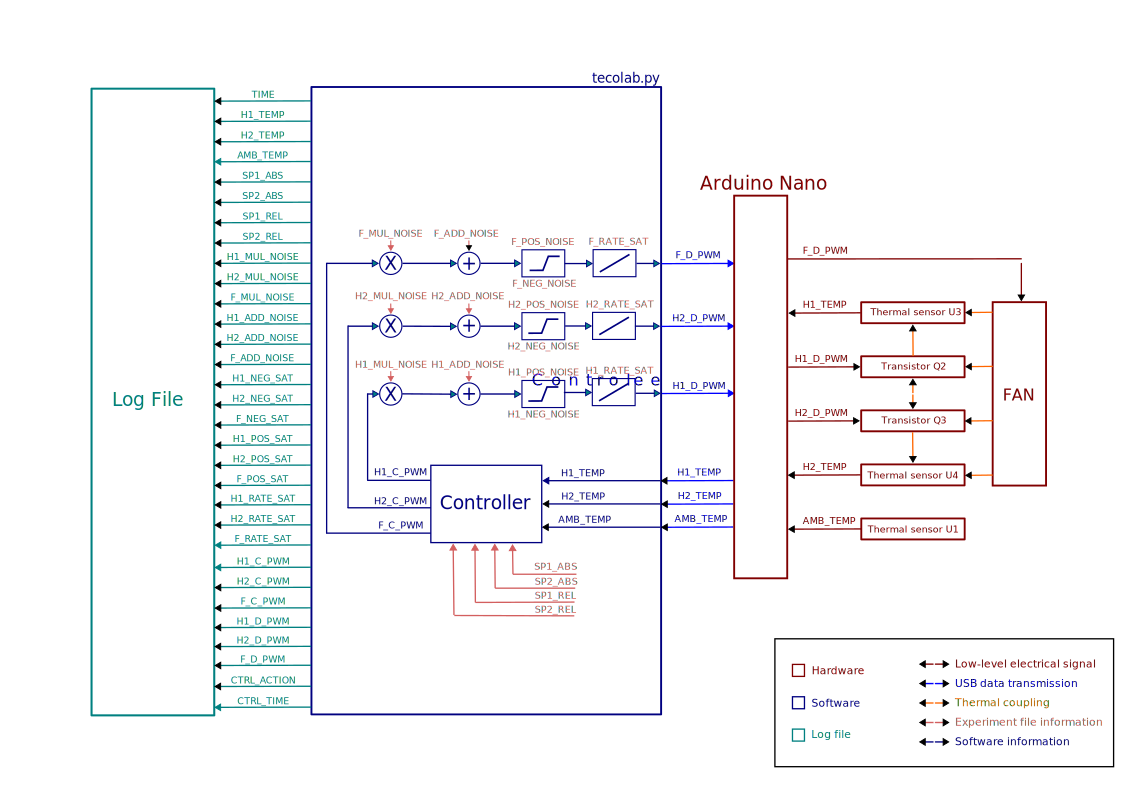
\includegraphics[scale = 0.53]{Figures/TeCoLabBlockDiagram.pdf}
\caption{Block Diagram of TeCoLab Experiment}\label{fig:TeCoLabBlockDiagram}
\end{figure}

The three types of files in TeCoLab are:

\begin{enumerate}
\item \textbf{Experiment File (\texttt{.csv}):} Located in \texttt{TeCoLab/Software/Experiments}. This file, provided by the user, defines the experiment setup, which includes details such as temperature setpoints, disturbances, and other parameters necessary for the description of the experiment. In the Figure~\ref{fig:TeCoLabBlockDiagram}, the experiment file is responsible to provide the information in pink. Refer to Section~\ref{sec:ExpFile} for a comprehensive guide on creating experiment files.


\item \textbf{Control File (\texttt{.py}):} Located in \texttt{TeCoLab/Software/Controllers}. This file, provided by the user, encapsulates the control algorithm for the experiment. Its purpose is to compute the control action for the two heaters and the fan based on the setpoints provided by the experiment file and the temperatures measurements from the board sensors. In the Figure~\ref{fig:StructureOfControlModules} the control file is represented by the \emph{Controller} block. Refer to Section~\ref{sec:ControlFile} for a comprehensive guide on creating control files. Observe that TeCoLab provides auxiliary scripts to help on the creation of various classical control algorithms, which are described in Chapter~\ref{chap:ControlTools}.

\item \textbf{Log File (\texttt{.csv}):} located in \texttt{TeCoLab/Software/Logs}. This file, created by the TeCoLab, contains detailed information about the experiment's execution, including timestamps, temperatures, and control actions. It is named with the date and time of the experiment. Refer to Section~\ref{sec:LogFile} for a comprehensive guide on creating interpreting log files.

\end{enumerate}

Understanding the roles and formats of these files is essential for effectively using TeCoLab. Consult the respective sections for each file type to ensure proper file creation and utilization.

\section{The Experiment File}\label{sec:ExpFile}

The Experiment File must be saved in \texttt{TeCoLab/Software/Experiments}. It is a CSV (Comma-Separated Values) which contains a detailed description of your experiment. The time indicated at the last row indicates the experiment's end in milliseconds (ms). For example, in the tutorial from Chapter~\ref{chap:getstarted}, the final value is 900000, equivalent to 15 minutes (900000 ms).

The columns of the Experiment File are explained as follows, with bold variables accessible to your control algorithm (see Section~\ref{sec:ControlFile} and Chapter~\ref{chap:ControlTools} for details):

\begin{itemize}
\item TIME: The time when this experiment row is applied (in ms);
\item \textbf{SP1\_ABS:} Absolute setpoint of Heater 1 (in °C);
\item \textbf{SP2\_ABS:} Absolute setpoint of Heater 2 (in °C);
\item \textbf{SP1\_REL:} Relative setpoint of Heater 1 (in °C);
\item \textbf{SP2\_REL:} Relative setpoint of Heater 2 (in °C);
\item H1\_MUL\_NOISE: Multiplicative noise for the control action of Heater 1 (dimensionless). The control action computed by the control algorithm is multiplied by this value. Default value is 1;
\item H2\_MUL\_NOISE: Multiplicative noise for the control action of Heater 2 (dimensionless). The control action computed by the control algorithm is multiplied by this value. Default value is 1;
\item F\_MUL\_NOISE: Multiplicative noise for the control action of the Fan (dimensionless). The control action computed by the control algorithm is multiplied by this value. Default value is 1;
\item H1\_ADD\_NOISE: Additive noise for the control action of Heater 1 (in \% of $P_{\text{max}}$). This value is added to the control action computed by the control algorithm. Default value is 0;
\item H2\_ADD\_NOISE: Additive noise for the control action of Heater 2 (in \% of $P_{\text{max}}$). This value is added to the control action computed by the control algorithm. Default value is 0;
\item F\_ADD\_NOISE: Additive noise for the control action of the Fan (in \% of $P_{\text{max}}$). This value is added to the control action computed by the control algorithm. Default value is 0;
\item H1\_NEG\_SAT: Negative saturation for the control action of Heater 1 (in \% of $P_{\text{max}}$). This represents the minimum possible value for the control action. Default value is 0;
\item H2\_NEG\_SAT: Negative saturation for the control action of Heater 2 (in \% of $P_{\text{max}}$). This represents the minimum possible value for the control action. Default value is 0;
\item F\_NEG\_SAT: Negative saturation for the control action of the Fan (in \% of $P_{\text{max}}$). This represents the minimum possible value for the control action. Default value is 0;
\item H1\_POS\_SAT: Positive saturation for the control action of Heater 1 (in \% of $P_{\text{max}}$). This represents the maximum possible value for the control action. Default value is 100;
\item H2\_POS\_SAT: Positive saturation for the control action of Heater 2 (in \% of $P_{\text{max}}$). This represents the maximum possible value for the control action. Default value is 100;
\item F\_POS\_SAT: Positive saturation for the control action of the Fan (in \% of $P_{\text{max}}$). This represents the maximum possible value for the control action. Default value is 100;
\item H1\_RATE\_SAT: Maximum rate of change for the control action of Heater 1 (in \% of $P_{\text{max}}$ per second). This represents the maximum possible rate of change for the control action. Default value is 1000;
\item H2\_RATE\_SAT: Maximum rate of change for the control action of Heater 2 (in \% of $P_{\text{max}}$ per second). This represents the maximum possible rate of change for the control action. Default value is 1000;
\item F\_RATE\_SAT: Maximum rate of change for the control action of the Fan (in \% of $P_{\text{max}}$ per second). This represents the maximum possible rate of change for the control action. Default value is 1000.
\end{itemize}

Note that there is no essential distinction among the parameters SP1\_ABS, SP2\_ABS, SP1\_REL and SP2\_REL. Your control algorithm can utilize the values specified in the experiment file for these fields according to your specific requirements.

\section{The Control File}\label{sec:ControlFile}

The control file in TeCoLab is a Python (\texttt{.py}) script in \texttt{TeCoLab/Software/Controllers}. Its primary purpose is to implement the control algorithm for your experiment. The control file interacts with the TeCoLab board to adjust the actuators (heaters and fan) based on the system's feedback.

Here are the steps to set up your control file from scratch (that is, without using the control scripts provided by TeCoLab, as explained in Chapter~\ref{chap:ControlTools}):

\begin{enumerate}
\item \textbf{Import the TeCoLab Default Controller Module}:

Begin your Python controller script by importing the default controller class from TeCoLab.
\begin{lstlisting}[language = Python]
from Modules.tecolab_controller import Controller
\end{lstlisting}

\item \textbf{Create a Class \texttt{Controller} that Inherits from \texttt{Controller}}:

Define a class named \texttt{Controller} in your Python script, inheriting from the default \texttt{Controller} class. This new class will be the blueprint for your custom control algorithm.

\begin{lstlisting}[language = Python, tabsize = 2]
class Controller(Controller):
	def __init__(self):
		super().__init__()
		# Create here your controller class attributes.
\end{lstlisting}

Thanks to the inheritance, your \texttt{Controller} class will have access to the following attributes:

\begin{itemize}
\item \texttt{setpoint\_abs\_1}: absolute setpoint temperature (in °C) for heater 1, obtained from the experiment file;
\item \texttt{setpoint\_abs\_2}: absolute setpoint temperature (in °C) for heater 2, obtained from the experiment file;
\item \texttt{setpoint\_rel\_1}: relative setpoint temperature (in °C) for heater 1, obtained from the experiment file;
\item \texttt{setpoint\_rel\_2}: relative setpoint temperature (in °C) for heater 2, obtained from the experiment file;
\item \texttt{temperature\_heater\_1}: measured temperature (in °C) for heater 1, obtained from the board sensors;
\item \texttt{temperature\_heater\_2}: measured temperature (in °C) for heater 2, obtained from the board  sensors;
\item \texttt{temperature\_ambient}: measured ambient temperature (in °C), obtained from the board sensors;
\item \texttt{actuator\_heater\_1}: control action for heater 1 (in \% of $P_{\text{max}}$), which will be applied to the board;
\item \texttt{actuator\_heater\_2}: control action for heater 2 (in \% of $P_{\text{max}}$), which will be applied to the board;
\item \texttt{actuator\_fan}: control action for the fan (in \% of $P_{\text{max}}$), which will be applied to the board;
\end{itemize}

If your control class uses a setpoint attribute whose value is not specified in the experiment file, an error will occur. For instance, if you utilize the attribute \texttt{self.setpoint\_abs\_2} in your control algorithm without specifying values in the column \texttt{SP2\_ABS} of the experiment file, an error will be triggered.

\item \textbf{Implement the \texttt{control\_setup()} Method}:

The \texttt{control\_setup()} method is executed once by TeCoLab at the start of your experiment. It's where you configure your controller, creating and setting up any specific attributes needed for your control algorithm. 

\begin{itemize}

\item \textbf{Parameters:} None;

\item \textbf{Returns:} None.

\item \textbf{Example:}
\begin{lstlisting}[language = Python]
def control_setup(self):
    # Your configuration code here
\end{lstlisting}

\end{itemize}
\item \textbf{Implement the \texttt{control\_action()} Method}:

The \texttt{control\_action()} method contains the computation of your control action. It must assign the calculated control actions to the following standard attributes from TeCoLab base controller class:
\begin{itemize}
\item \texttt{self.actuator\_heater\_1}
\item \texttt{self.actuator\_heater\_2}
\item \texttt{self.actuator\_fan}
\end{itemize}

If your control algorithm do not use some actuator (for example, the fan), no value need to be assigned for that attribute;

\begin{itemize}

\item \textbf{Parameters:} None;

\item \textbf{Returns:} None.

\item \textbf{Example:}
\begin{lstlisting}[language = Python]
def control_action(self):
    # Your control action computation code here
\end{lstlisting}

\end{itemize}
\item \textbf{Implement the \texttt{control\_signal()} Method}:

The \texttt{control\_signal()} method returns a boolean value. True means that a new control action must be computed, that is, the method \texttt{control\_action()} will be called in the current moment of the TeCoLab experiment. False means that a new control action will not be computed at this moment and, therefore, the last computed control action will be applied;

\begin{itemize}

\item \textbf{Parameters:} None;

\item \textbf{Returns:} Boolean;

\item \textbf{Example:}
\begin{lstlisting}[language = Python]
def control_signal(self):
    # Your control signal decision code here
    return True  # or False based on your logic
\end{lstlisting}
\end{itemize}
\end{enumerate}

Note: You don't have to build a controller file from scratch every time. TeCoLab provides tools that you can use. Refer to Chapter~\ref{chap:ControlTools} for more information.

\section{The Log File}\label{sec:LogFile}

The log file is a CSV (comma-separated values) file stored in the \texttt{TeCoLab/Software/Logs} folder. Its purpose is to register the results of your experiment. Each iteration of your experiment generates a new row in this file, with a default time interval of 200 milliseconds (configurable, see Chapter~\ref{chap:AdvancedConfigs}). The columns in the log file mirror those in the experiment file, with the following additional columns:

\begin{itemize}
\item H1\_TEMP: Current temperature of Heater 1 (in °C).
\item H2\_TEMP: Current temperature of Heater 2 (in °C).
\item AMB\_TEMP: Current ambient temperature (in °C).
\item H1\_C\_PWM: Computed value of the control action for Heater 1 (in \% of $P_{\text{max}}$).
\item H2\_C\_PWM: Computed value of the control action for Heater 2 (in \% of $P_{\text{max}}$).
\item F\_C\_PWM: Computed value of the control action for the fan (in \% of $P_{\text{max}}$).
\item H1\_D\_PWM: Disturbed value of the control action for Heater 1, accounting for multiplicative noise, additive noise, negative and positive saturation, and rate of change limitation (in \% of $P_{\text{max}}$).
\item H2\_D\_PWM: Disturbed value of the control action for Heater 2, accounting for multiplicative noise, additive noise, negative and positive saturation, and rate of change limitation (in \% of $P_{\text{max}}$).
\item F\_D\_PWM: Disturbed value of the control action for the fan, accounting for multiplicative noise, additive noise, negative and positive saturation, and rate of change limitation (in \% of $P_{\text{max}}$).
\item CTRL\_ACTION: A flag where the value 1 indicates whether a new control action was computed at that instant. If the value is 0, a new control action was not computed and the last computed control action was applied. This is equivalent to the return value of the \texttt{control\_signal()} method;
\item CTRL\_TIME: The time (in ms) taken to compute your control algorithm. This value can be useful for comparing the performance of different control algorithms.
\end{itemize}

\chapter{TeCoLab Control Tools}\label{chap:ControlTools}

TeCoLab provides Python scripts, referred to as \emph{modules}, designed to simplify the implementation of various classic control algorithms. These modules progressively introduce additional attributes, methods and functionalities to the \texttt{Controller} class in the structured manner displayed in Figure~\ref{fig:StructureOfControlModules}.

\begin{figure}[!htbp]
\centering
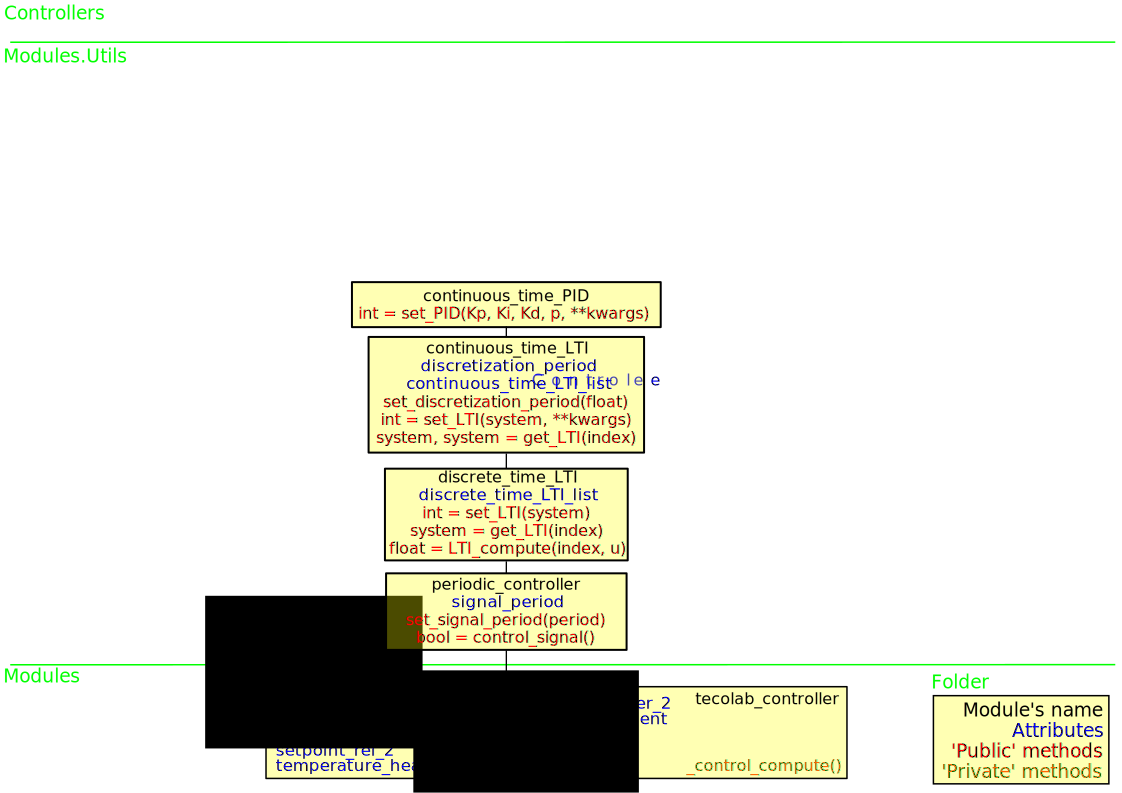
\includegraphics[scale = 0.55]{Figures/TeCoLabControlToolsDiagram.pdf}
\caption{Structure of the Control Modules.}\label{fig:StructureOfControlModules}
\end{figure}

The structure of Figure~\ref{fig:StructureOfControlModules} is divided in three layers, each one located in a different folder. The deepest layer can be found in \texttt{TeCoLab/Software/Modules} (the bottom one in Figure~\ref{fig:StructureOfControlModules}) and defines the base TeCoLab \texttt{Controller} class. Through its attributes, this class provides access to the values received from the TeCoLab board or that will be send to it. The middle layer is located in \texttt{TeCoLab/Sofware/Modules/Utils}. It provides tools to help you in the implementation of classical control algorithms, such as transfer functions. Finally, the last layer are the user's custom control scripts, which must be saved in \texttt{TeCoLab/Software/Controllers} and can use any module from the two layers below. Observe that you don't need to use the modules from the middle layer to build your control algorithms. What is important is that your control algorithm, through the use of modules or not, define three methods: \texttt{control\_signal()}, \texttt{control\_setup()} and \texttt{control\_action()} (see Section~\ref{sec:ControlFile} for details about these methods).

In the script file of each module, the code structure shown below is followed. The concept is that every script creates a class named \texttt{Controller}, inheriting from the imported \texttt{Controller} class from the previous module. It's crucial for each subsequent script, including your custom ones, to create a class with the identical name (\texttt{Controller}).

\begin{lstlisting}[language = Python]
from the_previous_module import Controller

class Controller(Controller):
	# Your control algorithm is coded inside this class.
\end{lstlisting}

\section{\texttt{tecolab\_controller} Module}

The \texttt{tecolab\_controller} module serves as the fundamental controller class in TeCoLab. Other classes build upon this base to provide additional attributes, methods and functionalities. This module defines the class \texttt{Controller}, which has attributes that receive values from the experiment table during the execution of an experiment, receive values from the sensors of the TeCoLab board or set values as control actions to the heaters and the fan. Next, the specifications of the class \texttt{Controller} defined by this module are given.

\begin{itemize}

\item Parameters: None

\item Attributes:

\begin{itemize}
\item \texttt{setpoint\_abs\_1} (float): Absolute setpoint temperature (in °C) for heater 1, obtained from the experiment file.

\item \texttt{setpoint\_abs\_2} (float): Absolute setpoint temperature (in °C) for heater 2, obtained from the experiment file.

\item \texttt{setpoint\_rel\_1} (float): Relative setpoint temperature (in °C) for heater 1, obtained from the experiment file.

\item \texttt{setpoint\_rel\_2} (float): Relative setpoint temperature (in °C) for heater 2, obtained from the experiment file.

\item \texttt{temperature\_heater\_1} (float): Measured temperature (in °C) for heater 1, obtained from the sensors.

\item \texttt{temperature\_heater\_2} (float): Measured temperature (in °C) for heater 2, obtained from the sensors.

\item \texttt{temperature\_ambient} (float): Measured ambiente temperature (in °C), obtained from the sensors.

\item \texttt{actuator\_heater\_1} (float): Control action for heater 1 (in \% of $P_{\text{max}}$), which will be applied by the TeCoLab software to the board.

\item \texttt{actuator\_heater\_2} (float): Control action for heater 2 (in \% of $P_{\text{max}}$), which will be applied by the TeCoLab software to the board.

\item \texttt{actuator\_fan}: Control action for the fan (in \% of $P_{\text{max}}$), which will be applied by the TeCoLab software to the board.
\end{itemize}

\item Methods:

\texttt{\_control\_compute(setPoints, temperatures)}:

Used by the TeCoLab to call other methods of the class during the experiment to compute the control actions. As a user, never use this method in your code.

\end{itemize}

To incorporate this module into your Python script, use the following line of code:

\begin{lstlisting}[language = Python]
from Modules.tecolab_controller import Controller
\end{lstlisting}

\section{\texttt{periodic\_controller} Module}

The \texttt{periodic\_controller} module builds upon the base controller class to facilitate the creation of periodic controllers within TeCoLab. These controllers compute new control actions at regular time intervals, defined by the period attribute \texttt{signal\_period}, which is added by this module. The period is given in multiples of the base period of a TeCoLab experiment, which is by default 200 ms (configurable, see Chapter~\ref{chap:AdvancedConfigs}). For instance, setting \texttt{signal\_period} to 5 results in a control action computed every 5 x 200 ms = 1 s. Next, the specifications of the class \texttt{Controller} defined by this module are given.

\begin{itemize}

\item Parameters: None

\item Attributes:

\begin{itemize}
\item \texttt{signal\_period} (int, default value 1): The period for computing control actions, specified in multiples of the base TeCoLab period.
\end{itemize}

\item Methods:

\texttt{set\_signal\_period(period)}:

Set the \texttt{signal\_period} attribute. It checks if the argument is a number, throwing an error if it is not. Moreover, if the argument is not an integer, it is rounded to the closest integer.

\begin{itemize}
\item Parameters:

\begin{itemize}
\item period (integer): The value to be assigned to the \texttt{signal\_period} attribute.
\end{itemize}

\item Returns: None

\end{itemize}

\texttt{control\_signal()}:

Computes the periodic control signal to determine whether a new control action should be computed. See Section~\ref{sec:ControlFile} for details about this method.

\end{itemize}

To incorporate this module into your Python script, use the following line of code:

\begin{lstlisting}[language = Python]
from Modules.Utils.periodic_controller import Controller
\end{lstlisting}

\section{\texttt{discrete\_time\_LTI} Module}

The \texttt{discrete\_time\_LTI} module provides the base class for creating controllers based on discrete-time Linear Time Invariant (LTI) systems, such as transfer functions or state space representations. It allows you to create LTI objects using the standard Python control library and store them within the \texttt{Controller} class. Then, you can compute the output of the stored LTI systems based on a given input. Next, the specifications of the class \texttt{Controller} defined by this module are given.

\begin{itemize}

\item Parameters: None

\item Attributes:

\begin{itemize}
\item \texttt{discrete\_time\_LTI\_list} (list, default value \emph{None}): The list of internally saved discrete-time LTI systems.
\end{itemize}

\item Methods:

\texttt{set\_LTI(system)}:

Store a discrete-time LTI system, which can be created using the TransferFunction or the StateSpace functions from Python standard control library. The method returns an integer representing the index of the stored LTI system, which is used to identify one specific system within the list of stored systems.

\begin{itemize}
\item Parameters:

\begin{itemize}
\item system (LTI): LTI object that can be created using the TransferFunction or the StateSpace functions from Python standard control library.
\end{itemize}

\item Returns:

\begin{itemize}

\item int: The index that identifies the stored LTI system.

\end{itemize}

\end{itemize}

\texttt{get\_LTI(index)}:

Get a previously stored discrete-time LTI system based on its index. The method returns the LTI system used for output computation in the state-space representation. Note that this representation is usually different from the original system stored (although equivalent).

\begin{itemize}
\item Parameters:

\begin{itemize}
\item index (int): The index that identifies the stored LTI system.
\end{itemize}

\item Returns:

\begin{itemize}

\item system (LTI): state space representation of the stored LTI object. This is the representation that the \texttt{Controller} class uses for output computation.

\end{itemize}

\end{itemize}

\texttt{LTI\_compute(index, u)}:

Computes the output of a previously created and stored LTI system.

\begin{itemize}
\item Parameters:

\begin{itemize}

\item index (int): The index that identifies the stored LTI system.

\item u (float): The input of the LTI system.

\end{itemize}

\item Returns:

\begin{itemize}

\item Float: The computed output of the LTI system.

\end{itemize}

\end{itemize}

\end{itemize}

To incorporate this module into your Python script, use the following line of code:

\begin{lstlisting}[language = Python]
from Modules.Utils.discrete_time_LTI import Controller
\end{lstlisting}

\section{\texttt{continuous\_time\_LTI} Module}

The \texttt{continuous\_time\_LTI} module provides the base class for creating controllers based on continuous-time LTI systems within TeCoLab. It allows you to create transfer functions or state space objects which are internally stored and then compute their output based on a given input. Note that, since TeCoLab is a digital plataform, the continuous-time LTI objects are later converted to discrete-time LTI objects in order to compute outputs. In order to have the correct behavior, your custom control algorithm should not change the \texttt{signal\_period} attribute, which will be automatically set to 1. Next, the specifications of the class \texttt{Controller} defined by this module are given.

\begin{itemize}

\item Parameters: None

\item Attributes:

\begin{itemize}
\item \texttt{discretization\_period} (float, default value 0.2): Period used in the discretization of the continuous-time LTI systems. To achieve the correct performance, this value must be equal to the TeCoLab iteration period (see Chapter~\ref{chap:AdvancedConfigs} for more information).

\item \texttt{continuous\_time\_LTI\_list} (list, default value \emph{None}): The list of internally saved continuous-time LTI systems.
\end{itemize}

\item Methods:

\texttt{set\_discretization\_period(period)}:

Set the discretization period used to convert the continuous-time LTI objects into discrete-time LTI objects. To achieve the correct performance, this value must be equal to the TeCoLab iteration period (see Chapter~\ref{chap:AdvancedConfigs} for more information).

\begin{itemize}
\item Parameters:

\begin{itemize}

\item period (float): Period used in the discretization process.

\end{itemize}

\item Returns: None.

\end{itemize}

\texttt{set\_LTI(system, **kwargs)}:

Store a continuous-time LTI system, which can be created using the TransferFunction or the StateSpace functions from Python standard control library. The method discretizes the continuous-time LTI system, stores it internally and returns an integer representing the index of the stored LTI system, which is used to identify one specific system within the list of stored systems.

\begin{itemize}
\item Parameters:

\begin{itemize}

\item system (LTI): continuous-time LTI object that can be created using the TransferFunction or the StateSpace functions from Python standard control library.

\item **kwargs: The additional arguments of the \texttt{control.sample\_system()} function from the standard Python control library.

\end{itemize}

\item Returns:

\begin{itemize}

\item int: The index that identifies the stored LTI system.

\end{itemize}

\end{itemize}

\texttt{get\_LTI(index)}:

Get a previously stored continuous-time LTI system and its discretized version based on its index. The method returns the two LTI systems.

\begin{itemize}
\item Parameters:

\begin{itemize}
\item index (int): The index that identifies the stored LTI system.
\end{itemize}

\item Returns:

\begin{itemize}

\item system (LTI): The original continuous-time LTI object stored.

\item system (LTI): The discretized LTI object. This is the representation used for computing the output of LTI objects.

\end{itemize}

\end{itemize}

\end{itemize}

To incorporate this module into your Python script, use the following line of code:

\begin{lstlisting}[language = Python]
from Modules.Utils.continuous_time_LTI import Controller
\end{lstlisting}

\section{\texttt{continuous\_time\_PID} Module}

The \texttt{continuous\_time\_PID} module provides the base class for creating continuous-time PID controllers. Next, the specifications of the class \texttt{Controller} defined by this module are given.

\begin{itemize}

\item Parameters: None

\item Attributes: None

\item Methods:

\texttt{set\_PID(Kp, Ki, Kd, p, **kwargs)}:

Creates a continuous-time PID transfer function and internally saves it. The PID format is given by
$$ C(s) = K_p\left(1 + \frac{K_i}{s} + sK_d\frac{p}{s+p}\right).$$

\begin{itemize}
\item Parameters:

\begin{itemize}

\item Kp (float): Proportional gain.

\item Ki (float): Integral gain.

\item Kd (float): Derivative gain.

\item p (float, default value 100): Pole for the low-pass filter used to make the derivative part causal.

\item **kwargs: The additional arguments of the \texttt{control.sample\_system()} function from the Python control module.

\end{itemize}

\item Returns:

\begin{itemize}

\item int: The index that identifies the stored LTI system.

\end{itemize}

\end{itemize}

\end{itemize}

To incorporate this module into your Python script, use the following line of code:

\begin{lstlisting}[language = Python]
from Modules.Utils.continuous_time_PID import Controller
\end{lstlisting}

\chapter{TeCoLab Advanced Configurations}\label{chap:AdvancedConfigs}

TeCoLab provides advanced configurations that can be specified as parameters when running the program from the terminal. These advanced configurations provide flexibility in adapting TeCoLab to specific requirements and computational constraints.

\section{Help}

To access the help menu for TeCoLab, use the following command:

\begin{lstlisting}[language = bash]
>> python3 tecolab.py -h
\end{lstlisting}

This command displays information about available options and how to use them.

\section{TeCoLab Experiment Period}\label{sec:TeCoLabPeriod}

You can adjust the base period of the TeCoLab experiment using the following command:

\begin{lstlisting}[language = bash]
>> python3 tecolab.py ExperimentFile ControlleFile -t XXX
\end{lstlisting}

Replace XXX with the desired period in milliseconds. For example, setting XXX to 500 means that an experiment iteration will occur every 500 ms, instead of the default 200 ms. Adjusting this period can be beneficial if your control algorithm's computation takes more than the default 200 ms. However, be cautious, as changing this value will also affect the period of control algorithms.


\chapter{FAQ - Frequently Asked Questions}\label{chap:FAQ}

\section{Why is the green LED blinking?}

The green LED blinks to indicate that the TeCoLab is awaiting the execution of a new experiment.

\section{Why is the green LED on?}

The green LED on indicates that the TeCoLab is currently executing an experiment.

\section{Why is the red LED blinking?}

The red LED blinks to indicate that the TeCoLab's heater elements are warm within a safe temperature range. Please avoid touching the heater elements when the red LED is blinking.

\section{Why is the red LED on?}\label{sec:RedLEDOn}

The red LED on indicates that the TeCoLab's heater elements are dangerously hot. In such a situation, TeCoLab will halt the current experiment and activate the fan to cool down the heater elements. It is crucial not to touch the heater elements when the red LED is on.

\section{Why the fan turned on without a command?}

See Section~\ref{sec:RedLEDOn}.

\section{Why the heaters are not heating?}

Check if you executed an experiment without connecting the 12 V DC power supply. In such case, the experiment will run normally, but without the power supply, the heaters and the fan will not activate.

\section{Why the time in log files are not equally spaced?}

Ideally, the time values in the log file should be evenly spaced, with a default spacing of 200 ms (see Section~\ref{sec:TeCoLabPeriod}). However, some variation (around 10 ms) is not uncommon.

If the variation is excessive, potential causes include:
\begin{itemize}
\item Your computer is overloaded: Try closing other applications or restarting your computer before running a TeCoLab experiment.
\item Your control algorithm takes too long: Check the control algorithm computation time in the log file (see Section~\ref{sec:LogFile}). If the time is excessive, consider optimizing your algorithm or adjusting the experiment period (see Chapter~\ref{chap:AdvancedConfigs}). Note: changing the experiment period may also impact your algorithm's execution period.
\end{itemize}

\section{Why a log file was not saved for my experiment?}

An experiment must run for more than 5 seconds to save a log file.

\section{Why don't all the temperatures match at the beginning of the experiment?}

A slight temperature difference (around 1 °C) between the initial heater temperatures and the ambient temperature is common due to sensor variations. If the difference is greater, ensure you are not running consecutive experiments. After one experiment, wait for sufficient time for the heater elements to cool down before starting another one.

\section{Why the temperature experienced a non specified disturbance?}

Note that TeCoLab is a physical system, which means that external disturbances, not specified in the experiment file, might affect its sensors. For example, if a gust of wind blows on TeCoLab's temperature sensors, it can introduce unexpected disturbances. To prevent such scenarios, it is recommended to run TeCoLab experiments in an environment where the system will not be subject to external disturbances.

\end{document}